\capitulo{5}{Aspectos relevantes del desarrollo del proyecto}



\section{Análisis evolutivo de las redes de dependencias de repositorios de paquetes}

\subsection{La red de dependencias de PyPI}

En el ámbito del lenguaje de programación \textit{Python}, nos enfocamos en el análisis de \textit{PyPI}
(\textit{Python Package Index}). \textit{PyPI} es un repositorio ampliamente adoptado en la comunidad de
\textit{Python} debido a su facilidad de uso, su naturaleza de código abierto y su extensa colección de
paquetes.\footnote{Es importante mencionar que existen otros repositorios interesantes como \textit{Conda}.}

La facilidad de uso de \textit{PyPI} se deriva de su diseño intuitivo y las funcionalidades que ofrece
para la gestión de paquetes en \textit{Python}. Los desarrolladores pueden acceder a \textit{PyPI} como
una fuente centralizada para descubrir, descargar e instalar una amplia variedad de paquetes y bibliotecas
desarrollados por la comunidad.

En el análisis comparativo entre los datos proporcionados por \textit{libraries.io} y los recolectados en
este trabajo, se ha revelado una sorprendente tendencia en el número de paquetes presentes en \textit{PyPI}.
Se ha observado un aumento significativo en la cantidad de paquetes disponibles en \textit{PyPI} en
comparación con datos anteriores (en concreto un 474 \% ).

Este hallazgo sugiere un crecimiento notable en el ecosistema de paquetes de \textit{Python} y evidencia
el interés y participación de la comunidad en \textit{PyPI}. Este aumento en el número de paquetes puede
ser atribuido a diversos factores, como la creciente popularidad de \textit{Python} como lenguaje de
programación, el aumento en la adopción de \textit{Python} en diferentes campos de aplicación y el
creciente número de contribuyentes que comparten sus proyectos y soluciones a través de \textit{PyPI}.


\begin{figure}[ht]
    \begin{center}
        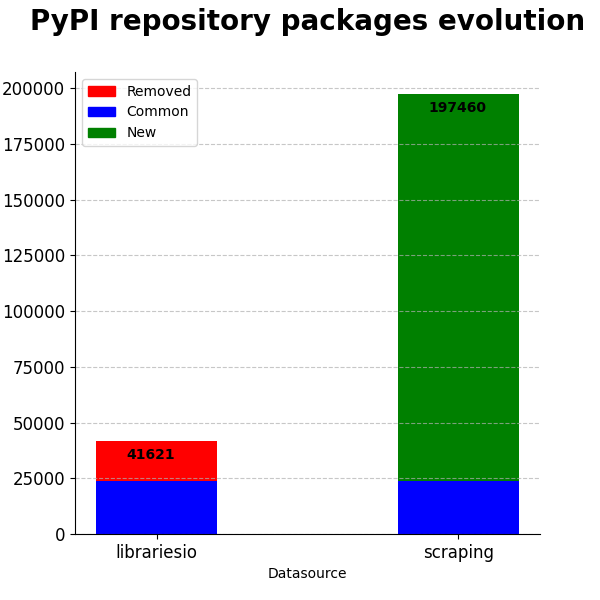
\includegraphics[width=0.6\textwidth]{/home/dnllns/Documentos/repositorios/olivia-finder-memoria/img/pypi/bar_common_packages.png}
        \caption{Comparacion de la cantidad de paquetes en PyPI entre los datos de libraries.io y los recolectados en este trabajo.}
        \label{fig:etiqueta}
        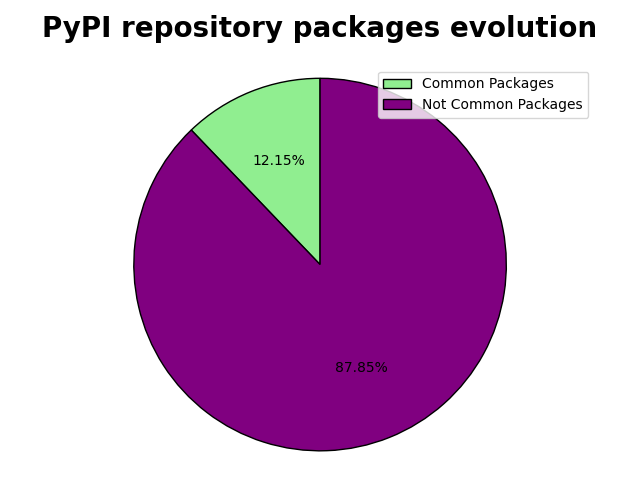
\includegraphics[width=0.6\textwidth]{/home/dnllns/Documentos/repositorios/olivia-finder-memoria/img/pypi/circ_common_packages.png}
        \caption{Paquetes comunes y no comunes actualmente.}
        \label{fig:pipy_common_packages_circle}
    \end{center}
\end{figure}

\begin{table}[t!]
    \begin{center}
        \begin{tabular}{|l|r|}
            \hline
            \textbf{Descripción}                               & \textbf{Cantidad} \\
            \hline
            Paquetes en libraries.io                           & 41,621            \\
            Paquetes en scraped                                & 197,460           \\
            Paquetes comunes                                   & 24,001            \\
            Paquetes de libraries.io no disponibles en scraped & 17,620            \\
            Paquetes en scraped que no estan en libraries.io   & 173,459           \\
            \hline
        \end{tabular}
    \end{center}
\end{table}


El análisis de los datos revela que aproximadamente el \textit{57 \%} de los paquetes que estaban
presentes en el conjunto de datos antiguo de PyPI se han mantenido en el nuevo conjunto de datos
\footnote{Este porcentaje se basa en datos obtenidos experimentalmente.}. Este porcentaje
relativamente elevado indica que la red de paquetes en PyPI ha logrado mantener una cantidad considerable
de paquetes de manera estable a lo largo del tiempo.

Es importante destacar que este conjunto de paquetes que se ha mantenido representa aproximadamente
el \textit{12.15\%} del total de paquetes disponibles en PyPI en la actualidad. Esta proporción nos
proporciona una idea de la estabilidad relativa de la red, ya que una parte significativa de los
paquetes ha logrado mantener su presencia en PyPI a pesar de los posibles cambios y
actualizaciones\footnote{Los datos se refieren al momento de la última actualización y pueden estar
    sujetos a cambios futuros.}.

\begin{figure}[ht]
    \begin{center}
        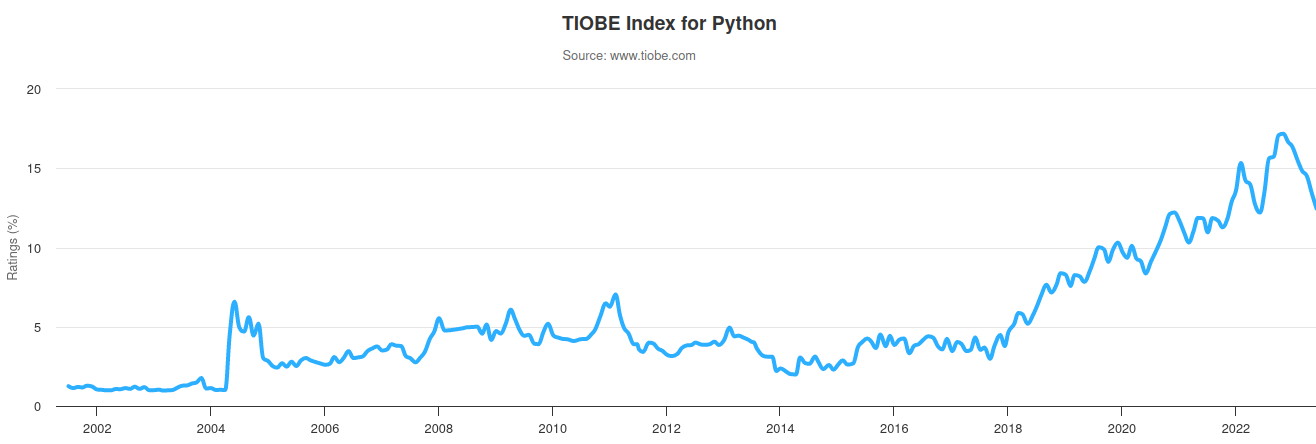
\includegraphics[width=1\textwidth]{/home/dnllns/Documentos/repositorios/olivia-finder-memoria/img/pypi/pypi_popularity.png}
        \caption{Popularidad de PyPI a lo largo del tiempo.}
        \label{fig:pypi_popularity}
    \end{center}
\end{figure}


Esta tendencia en la popularidad de Python se ve reflejada en las estadísticas realizadas por la
empresa TIOBE\footnote{\url{https://www.tiobe.com/tiobe-index/python/}}.


\subsubsection{Grado de la red}

Al examinar la distribución de grado en ambos conjuntos de datos, se observa que sigue una distribución
de ley de potencias\footnote{La distribución de ley de potencias es una característica común en las redes
    de dependencias.}.

Al analizar el gráfico, se evidencia que el grado máximo alcanzado por un paquete ha
experimentado un incremento significativo. Tomando como punto de referencia el número de nodos con grado
\textit{1000}, se puede apreciar una diferencia sustancial entre la red de \textit{libraries.io} y los
nuevos datos recolectados. Mientras que en \textit{libraries.io} se registran menos de \textit{10} paquetes
con dicho grado, en los nuevos datos se han identificado aproximadamente \textit{40} individuos
\footnote{Estos datos se basan en el análisis realizado en una fecha específica y pueden estar sujetos
    a cambios en el tiempo.}.

\begin{figure}[h!]
    \begin{center}
        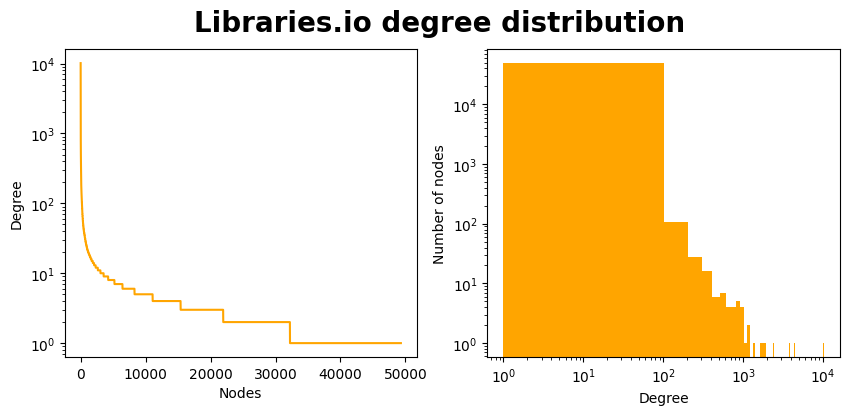
\includegraphics[width=0.8\textwidth]{img/pypi/librariesio_degree_distribution.png}
        \caption{Distribucion de grado de PyPI para libraries.io.}
        \label{fig:pypi_librariesio_degree_distribution}
    \end{center}
\end{figure}

\begin{figure}[h!]
    \begin{center}
        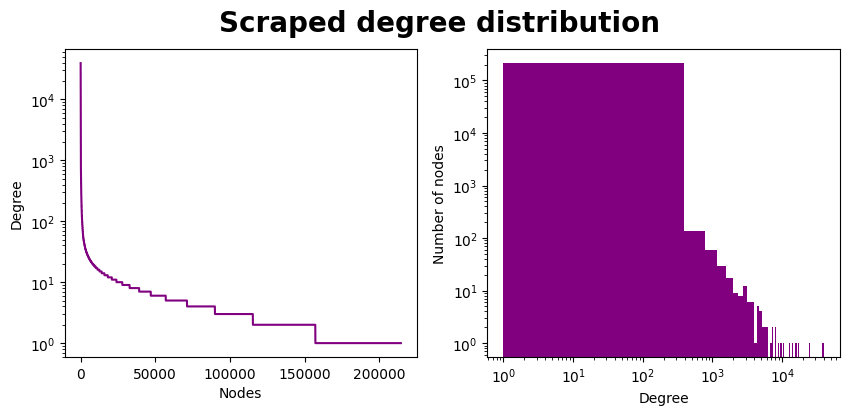
\includegraphics[width=0.8\textwidth]{img/pypi/scraped_degree_distribution.png}
        \caption{Distribucion de grado de PyPI para los datos recolectados.}
        \label{fig:pypi_scraped_degree_distribution}
    \end{center}
\end{figure}

Además, al calcular el grado promedio de los grafos correspondientes a \textit{libraries.io} y el nuevo
conjunto, se obtiene un valor de \textit{2.73} y \textit{4.35}, respectivamente. Estos valores indican
que, en promedio, cada paquete en la red de \textit{libraries.io} está conectado a alrededor de
\textit{2.73} otros paquetes, mientras que en los nuevos datos, cada paquete está conectado a
aproximadamente \textit{4.35} otros paquetes\footnote{Estos cálculos se realizaron utilizando una
    metodología específica y pueden variar dependiendo de la definición de conexión utilizada.}.

Estas estadísticas revelan cambios importantes en la estructura de la red de dependencias de paquetes.
El incremento en el grado máximo y el aumento en el grado promedio indican una mayor interconectividad
y complejidad en la red, lo cual puede ser atribuido al crecimiento y la evolución del ecosistema de
paquetes en Python.

Es importante destacar que la distribución de ley de potencias y la presencia de paquetes con grados
altos en la red tienen implicaciones significativas en términos de la propagación de dependencias y la
influencia de ciertos paquetes en la comunidad\footnote{Estas implicaciones pueden afectar la
    estabilidad, la modularidad y la confiabilidad del ecosistema de paquetes en Python.}.

\textbf{Grado de salida (\textit{out degree})}

El \textit{out degree} es una métrica que nos proporciona información
sobre el número de dependientes de un paquete dado. En el contexto de \textit{libraries.io},
analizando los datos, podemos identificar los paquetes que tienen más dependencias, es decir,
los que están en el \textit{Top} de las dependencias más utilizadas.


Los resultados obtenidos revelan una tendencia general en la cual las dependencias más populares han
experimentado un aumento en su popularidad, siendo ahora requeridas por un mayor número de paquetes
en la red de dependencias. En particular, se observa un incremento significativo en la popularidad
de las bibliotecas \textit{requests}, \textit{numpy}, \textit{pandas} y \textit{pytest} en comparación
con otros paquetes presentes en este ranking.

Estos hallazgos indican que estas bibliotecas han adquirido una mayor relevancia y utilidad en el
desarrollo de proyectos y aplicaciones en el entorno de Python. 

\begin{figure}[h!]
    \begin{center}
        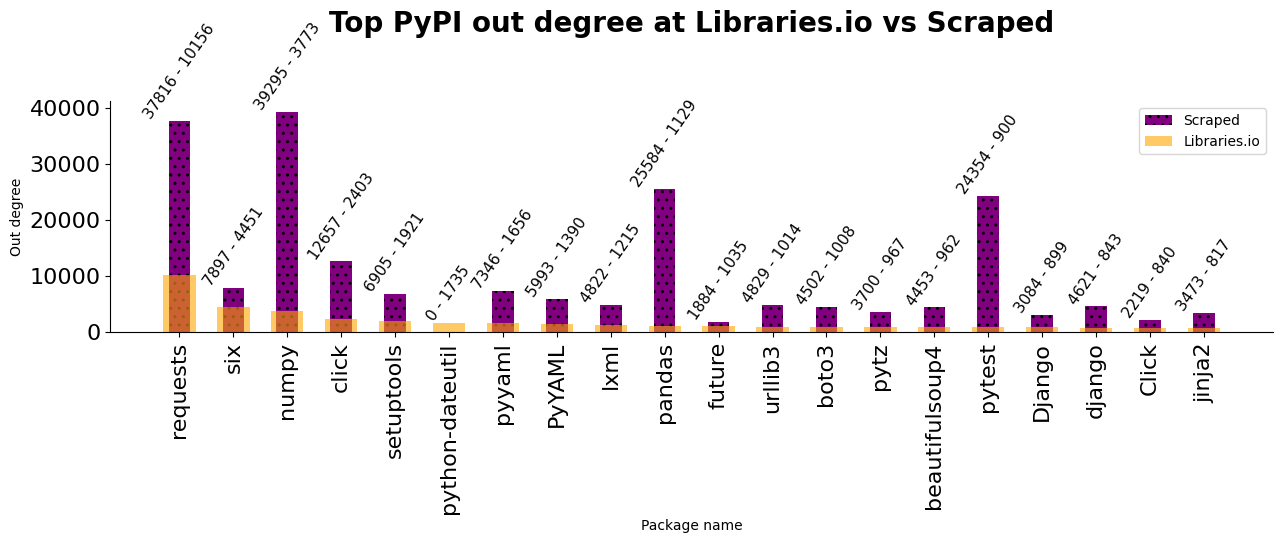
\includegraphics[width=1\textwidth]{/home/dnllns/Documentos/repositorios/olivia-finder-memoria/img/pypi/libio_t20_outd_comparison.png}
        \caption{Top de paquetes con mayor grado de salida en PyPI para libraries.io }
        \label{fig:pypi_libio_outd_comparison}
    \end{center}
\end{figure}

\begin{figure}[h!]
    \begin{center}
        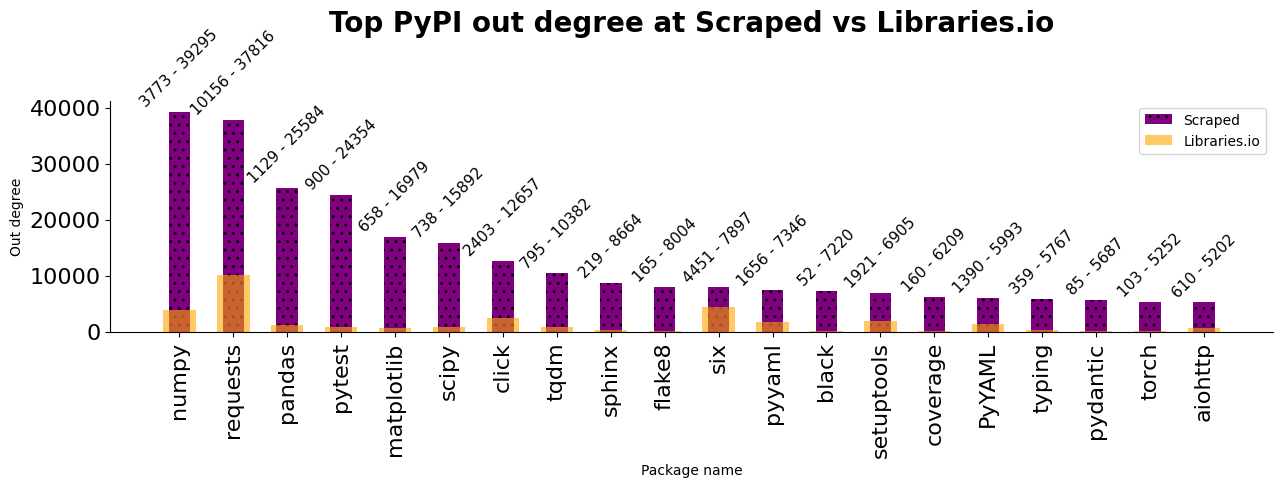
\includegraphics[width=1\textwidth]{/home/dnllns/Documentos/repositorios/olivia-finder-memoria/img/pypi/libio_scraped_t20_comparation.png}
        \caption{Top de paquetes con mayor grado de salida en PyPI para scraped.}
        \label{fig:pypi_scraped_outd_comparison}
    \end{center}
\end{figure}

En este análisis de ranking, se observa que ciertos paquetes se han mantenido con respecto al ranking
anterior, lo cual indica su relevancia a lo largo del tiempo. Estos
paquetes incluyen \textit{PyYAML}, \textit{click}, \textit{numpy}, \textit{pandas}, \textit{pytest},
\textit{pyyaml}, \textit{requests}, \textit{setuptools} y \textit{six}. Su presencia continua en el
ranking sugiere que son dependencias fundamentales y ampliamente utilizadas en proyectos y aplicaciones
de Python\footnote{La relevancia y utilidad de estos paquetes se basa en la percepción de la comunidad
    de desarrolladores de Python y puede variar dependiendo del contexto y los requisitos del proyecto}.

Por otro lado, se identifican paquetes que han ascendido en el ranking en comparación con la clasificación
anterior. Estos paquetes incluyen \textit{black}, \textit{coverage}, \textit{flake8}, \textit{matplotlib},
\textit{odoo}, \textit{python}, \textit{scikit}, \textit{scipy}, \textit{sphinx}, \textit{tqdm} y
\textit{typing}. Su ascenso en el ranking puede ser atribuido a su creciente popularidad y utilidad en el
desarrollo de proyectos de Python, ya que son bibliotecas ampliamente conocidas y utilizadas por la
comunidad de desarrolladores\footnote{El ascenso en el ranking puede deberse a mejoras en funcionalidad,
    adopción en proyectos populares u otros factores que influyen en su popularidad}.

Por último, se muestra la distribución de \textit{out degree} para ambos conjuntos de datos \ref{fig:pypi_libio_outd_dist} \ref{fig:pypi_scraped_outd_dist}

\begin{figure}[h!]
    \begin{center}
        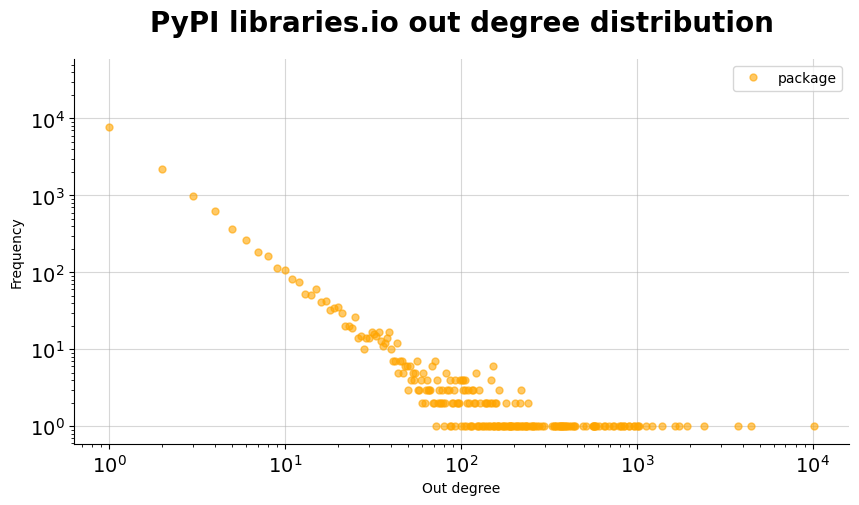
\includegraphics[width=0.8\textwidth]{/home/dnllns/Documentos/repositorios/olivia-finder-memoria/img/pypi/outd_libio_dist.png}
        \caption{Distribución de \textit{Out degree} para libraries.io}
        \label{fig:pypi_libio_outd_dist}
    \end{center}
\end{figure}

\begin{figure}[h!]
    \begin{center}
        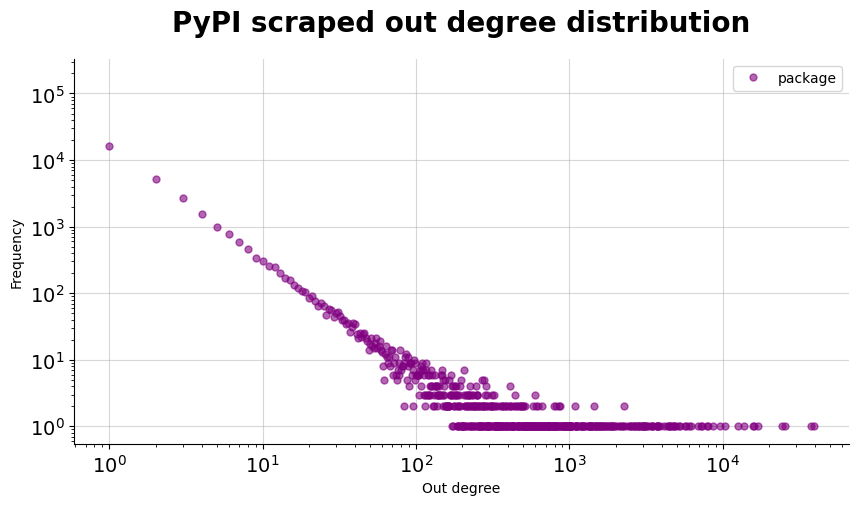
\includegraphics[width=0.8\textwidth]{/home/dnllns/Documentos/repositorios/olivia-finder-memoria/img/pypi/outd_scraped_dist.png}
        \caption{Distribución de \textit{Out degree} para scraped}
        \label{fig:pypi_scraped_outd_dist}
    \end{center}
\end{figure}

Al analizar los gráficos de las distribuciones de \textit{out degree}, se observa una tendencia similar
en ambos conjuntos. Se evidencia un incremento general en el número total de paquetes, lo que indica un
crecimiento continuo en el ecosistema de paquetes.

Se ha observado un aumento en el número de paquetes con un grado de salida bajo, lo que indica que estos
paquetes tienen menos dependencias externas. Este fenómeno puede deberse a la introducción de paquetes
más autónomos y autosuficientes en el ecosistema de Python, lo que reduce la necesidad de depender de
otros paquetes para su funcionamiento.

Por otro lado, se ha identificado un incremento \ref{fig:dependents_increase} en el grado de salida de los paquetes más populares.
Esto indica que estos paquetes están siendo cada vez más utilizados como dependencias por otros paquetes
en la comunidad de Python. Este aumento en el grado de salida de los paquetes populares puede ser atribuido
a su funcionalidad ampliamente reconocida y popularidad.

\begin{figure}[h!]
    \begin{center}
        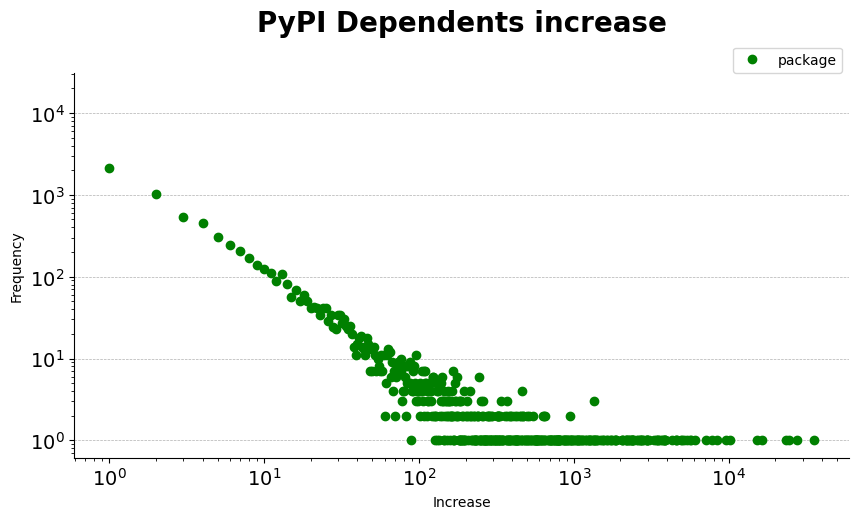
\includegraphics[width=0.8\textwidth]{/home/dnllns/Documentos/repositorios/olivia-finder-memoria/img/pypi/dependents_increase.png}
        \caption{Incremento del \textit{Out degree} en PyPI}
        \label{fig:dependents_increase}
    \end{center}
\end{figure}


\textbf{Grado de entrada (\textit{In degree})}

Esta métrica nos da una idea del número de dependencias que tiene un paquete dado.
Analizados los datos de libraries.io y representados sobre un grafico obtenemos los siguientes resultados: \ref{fig:pypi_libio_ind_comparison}

\begin{figure}[h!]
    \begin{center}
        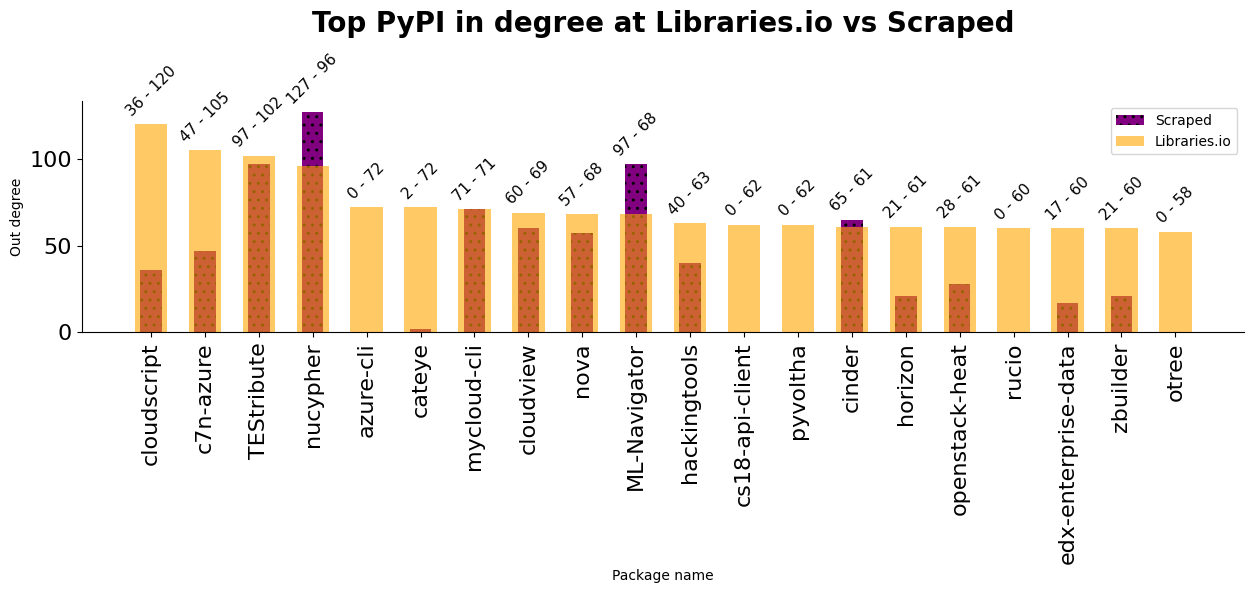
\includegraphics[width=1\textwidth]{/home/dnllns/Documentos/repositorios/olivia-finder-memoria/img/pypi/libio_t20_ind_comparison.png}
        \caption{Top paquetes con mayor \textit{In degree} en libraries.io}
        \label{fig:pypi_libio_ind_comparison}
    \end{center}
\end{figure}

Se observa una tendencia decreciente en el número de dependencias entre los paquetes con mayor In degree
dentro del conjunto de bibliotecas de \textit{libraries.io}, lo cual sugiere una inclinación natural de los
paquetes hacia una disminución de las dependencias requeridas. Además, se aprecia que una proporción significativa
de estos paquetes, caracterizados por una elevada cantidad de dependencias, ha experimentado una desaparición,
representando aproximadamente un 25 \% de las instancias evaluadas. Por consiguiente, se puede inferir que,
en general, la presencia de un alto número de dependencias no suele correlacionarse con la estabilidad de
los paquetes en el repositorio.

\begin{figure}[h!]
    \begin{center}
        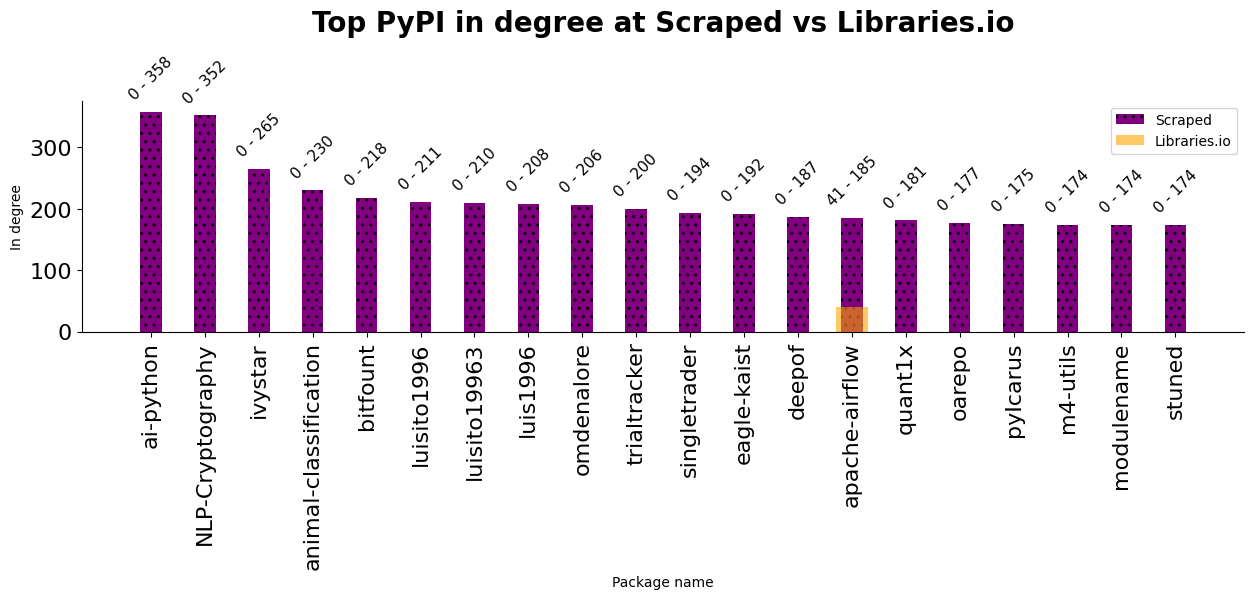
\includegraphics[width=1\textwidth]{/home/dnllns/Documentos/repositorios/olivia-finder-memoria/img/pypi/scraped_t20_ind_comparison.png}
        \caption{Top paquetes con mayor \textit{In degree} en scraped}
        \label{fig:pypi_scraped_ind_comparison}
    \end{center}
\end{figure}

Si realizamos este mismo análisis con el top 20 de los paquetes con más \textit{In degree} en la actualidad \ref{fig:pypi_scraped_ind_comparison}, podemos llegar a
conclusiones similares. Se observa una tendencia decreciente en el número de dependencias de los paquetes
más influyentes, lo cual sugiere una reducción en la cantidad de paquetes que dependen directamente de ellos.
Esto puede indicar cambios en las estrategias de desarrollo, la aparición de alternativas o la evolución de la
comunidad de desarrolladores.

Estos hallazgos resaltan la importancia de considerar tanto el In degree como el grado de salida de
los paquetes al analizar la estabilidad y la evolución de la red de dependencias en el ecosistema de Python.

Como se puede apreciar, el \textit{95 \%} de los paquetes pertenecientes a este conjunto presentan una ausencia
de dependencias.
Si profundizamos en el tema, podemos apreciar que estos paquetes son de reciente aparición. La falta de
dependencias en los paquetes puede ser resultado de su diseño modular, el uso de
bibliotecas internas o la falta de necesidad de dependencias externas.

Cabe destacar un caso particular, el paquete denominado \textit{apache-airflow}
\footnote{\url{https://pypi.org/project/apache-airflow/}}, el cual ha experimentado un considerable aumento
en el número de dependencias, pasando de 41 a 185. La explicación que se atribuye a este fenómeno es la
incorporación de nuevas funcionalidades, dado que se trata de un paquete con cierta popularidad. No obstante,
desde la perspectiva del autor de este Trabajo Final de Grado, se recomienda a los desarrolladores reducir
al máximo este número de dependencias para mejorar su estabilidad\footnote{El aumento en el número de dependencias
    puede aumentar la complejidad y la posibilidad de conflictos en el entorno de desarrollo. Se sugiere evaluar
    cuidadosamente las dependencias necesarias y buscar alternativas más ligeras o mejor optimizadas si es posible}.

\begin{figure}[h!]
    \begin{center}
        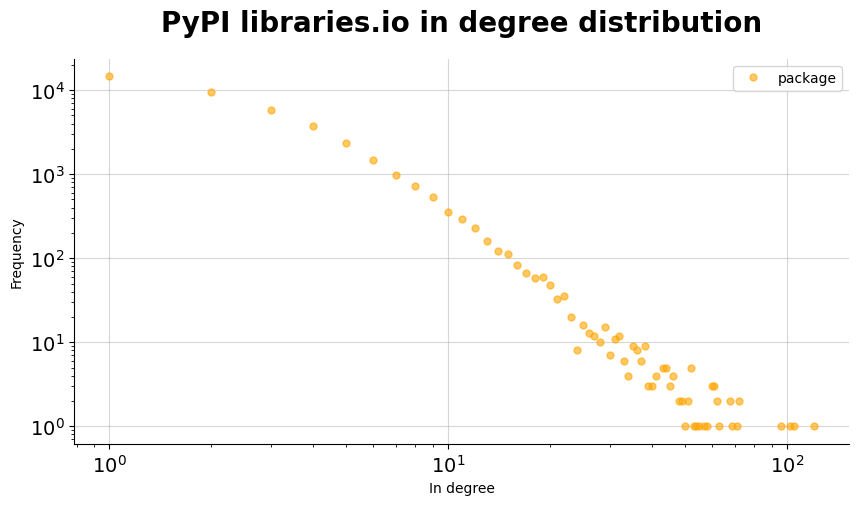
\includegraphics[width=0.8\textwidth]{/home/dnllns/Documentos/repositorios/olivia-finder-memoria/img/pypi/ind_libio_d.png}
        \caption{Distribucion del \textit{In degree} en libraries.io}
        \label{fig: Distribucion del In degree en libraries.io}
    \end{center}
\end{figure}

\begin{figure}[h!]
    \begin{center}
        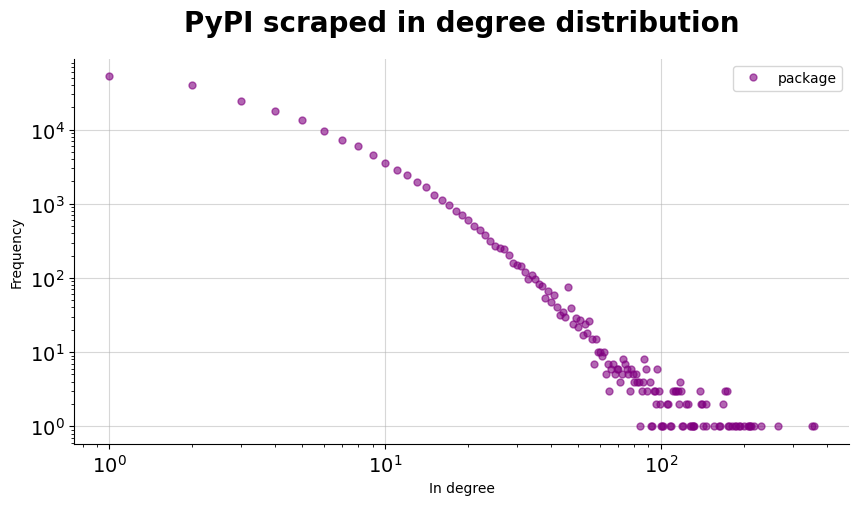
\includegraphics[width=0.8\textwidth]{/home/dnllns/Documentos/repositorios/olivia-finder-memoria/img/pypi/ind_scraped_dist.png}
        \caption{Distribucion del \textit{In degree} en scraped}
        \label{fig: Distribucion del In degree en scraped}
    \end{center}
\end{figure}

En el análisis de la distribución de In degree \ref{fig: Distribucion del In degree en libraries.io}, 
se ha observado una alta frecuencia de nodos con un bajo grado,
lo que indica la presencia de numerosos paquetes que no son utilizados como dependencias. Además, se ha identificado
una clara tendencia descendente en la frecuencia a medida que aumenta el \textit{In degree}.
Esto claramente representa una \textit{distribucion Power Law} \cite{enwiki:1160892030}.

La disminución en la frecuencia se vuelve significativa a medida que se alcanza un \textit{In degree} del orden
de $10^2$, donde la frecuencia se reduce a un único nodo por caso. Esto implica que existe una disminución drástica
en la cantidad de paquetes con un \textit{In degree} alto, lo cual sugiere que son menos comunes aquellos paquetes
que son ampliamente utilizados como dependencias por otros.

Si observamos la evolución \ref{fig: Distribucion del In degree en scraped}, se observa una tendencia similar en ambos casos, aunque en el estado actual se evidencia
un aumento en el número de nodos. La forma de la distribución se mantiene similar, pero se aprecia un considerable
incremento en el \textit{In degree}. Si consideramos la conclusión anteriormente obtenida, podemos constatar que
también se cumple en este caso, dado que el incremento en la frecuencia implica una disminución en el grado de
entrada.

\subsubsection{Pagerank}

La métrica de \textit{PageRank}\footnote{PageRank es un algoritmo utilizado para establecer un ranking de importancia en la web.}
nos permite establecer un ranking de importancia respecto a los paquetes. A la vista de la distribución obtenida de la red
de \textit{libraries.io}, una conclusión que se puede extraer es que la mayoría de las dependencias no son consideradas
importantes, ya que pertenecen al primer grupo, con una frecuencia considerablemente alta pero una baja relevancia en
términos de \textit{PageRank}. Sin embargo, existe un grupo más reducido pero significativo que presenta una importancia
media, pero son relevantes a nivel de que tienen múltiples enlaces provenientes de diferentes paquetes. Estas dependencias
comunes desempeñan un papel crítico en la interconexión de los diferentes componentes de la red. Además, se destaca
la presencia de un conjunto selecto de dependencias con un alto \textit{PageRank}, lo que indica su gran popularidad
y relevancia en la red de paquetes. En este grupo, las dependencias son enlazadas por muchas otras dependencias,
pero no tienen dependencias propias.

En concreto, estas son las dependencias más importantes a tener en cuenta debido a que suelen ser común su
aparición \ref{fig:Top 20 pagerank en libraries.io}.

\begin{figure}[h!]
    \begin{center}
        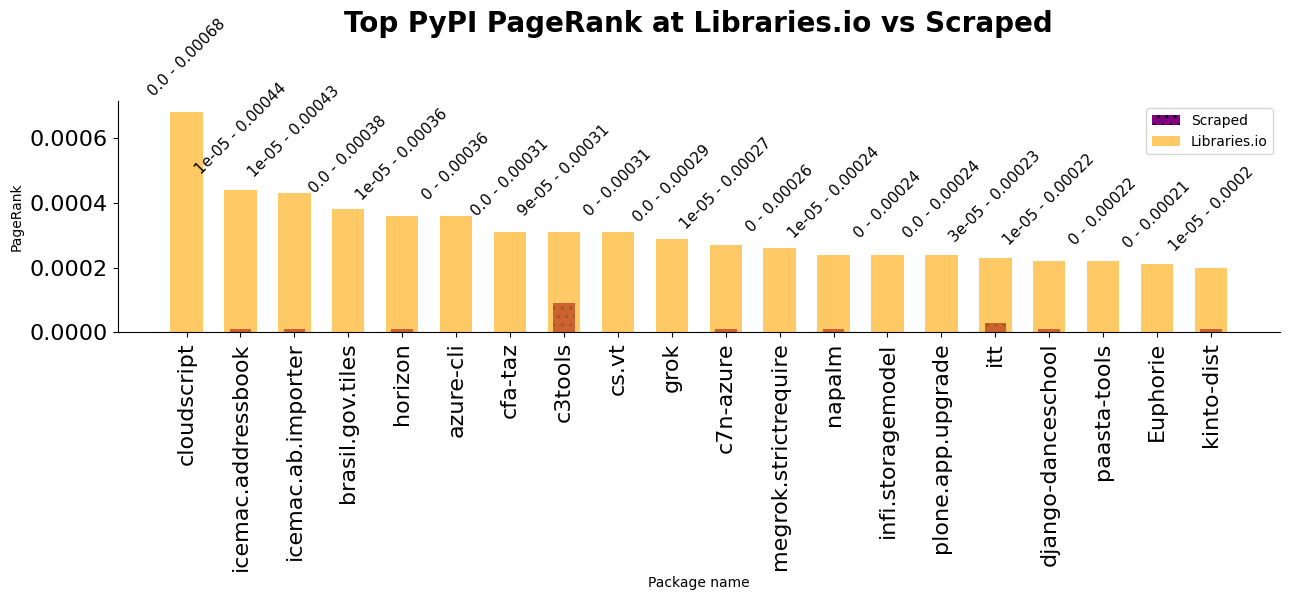
\includegraphics[width=1\textwidth]{img/pypi/libio_t20_pr_comparison.png}
        \caption{Top 20 \textit{PageRank} en libraries.io}
        \label{fig:Top 20 pagerank en libraries.io}
    \end{center}
\end{figure}

En términos de vulnerabilidad, los paquetes más críticos son aquellos que, si experimentan problemas o inestabilidad,
pueden tener un impacto significativo en toda la red de dependencias. Una dependencia crítica con múltiples enlaces
entrantes puede generar la propagación de errores o vulnerabilidades a través de los paquetes que dependen de
ella\footnote{Una dependencia crítica es aquella que, al presentar problemas, puede afectar negativamente a
    otros paquetes que dependen de ella, causando errores o vulnerabilidades en cadena.}.

Si visualizamos el número de dependencias transitivas \ref{fig:Dependencias transitivas del top 20 pagerank en libraries.io}
de estos paquetes, podemos obtener conclusiones más precisas.
Existe un grupo de paquetes con un menor número de dependencias transitivas, lo que los hace menos vulnerables en
comparación con el resto. Además, tener un alto \textit{PageRank} en estos paquetes implica que son más confiables
en términos de dependencias\footnote{Un paquete con un alto \textit{PageRank} y un bajo número de dependencias
    transitivas es considerado confiable y menos propenso a problemas de vulnerabilidad, ya que su estructura de
    dependencias es más simple y controlada.}.

\begin{figure}[h!]
    \begin{center}
        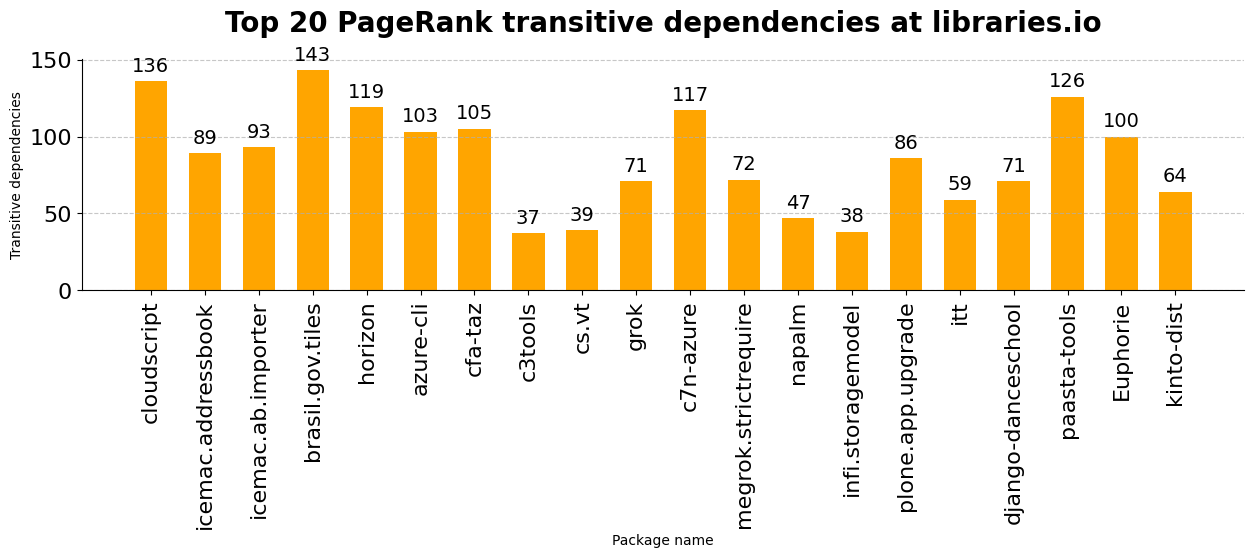
\includegraphics[width=1\textwidth]{img/pypi/transitive libraries.png}
        \caption{Dependencias transitivas del top 20 \textit{PageRank} en libraries.io}
        \label{fig:Dependencias transitivas del top 20 pagerank en libraries.io}
    \end{center}
\end{figure}

También se observa que en este grupo de paquetes, las dependencias transitivas son en promedio
más bajas\footnote{El número de dependencias transitivas en este grupo de paquetes tiende a
    ser menor en comparación con otros grupos, lo que indica una estructura más ligera y menos
    compleja en términos de dependencias.}.

Al analizar los resultados, se puede ver que los paquetes presentes en este grupo han
experimentado una evolución considerable \ref{fig:Top PageRank en scraped}, con una reducción significativa en
su \textit{PageRank}\footnote{El \textit{PageRank} de estos paquetes ha disminuido
    en comparación con mediciones anteriores.}. Esto se explica por la desaparición de algunos
de estos paquetes, la aparición de otros nuevos que han reemplazado su importancia y
la evolución de los propios paquetes hacia una mayor estabilización, lo que ha disminuido
su vulnerabilidad.

\begin{figure}[h!]
    \begin{center}
        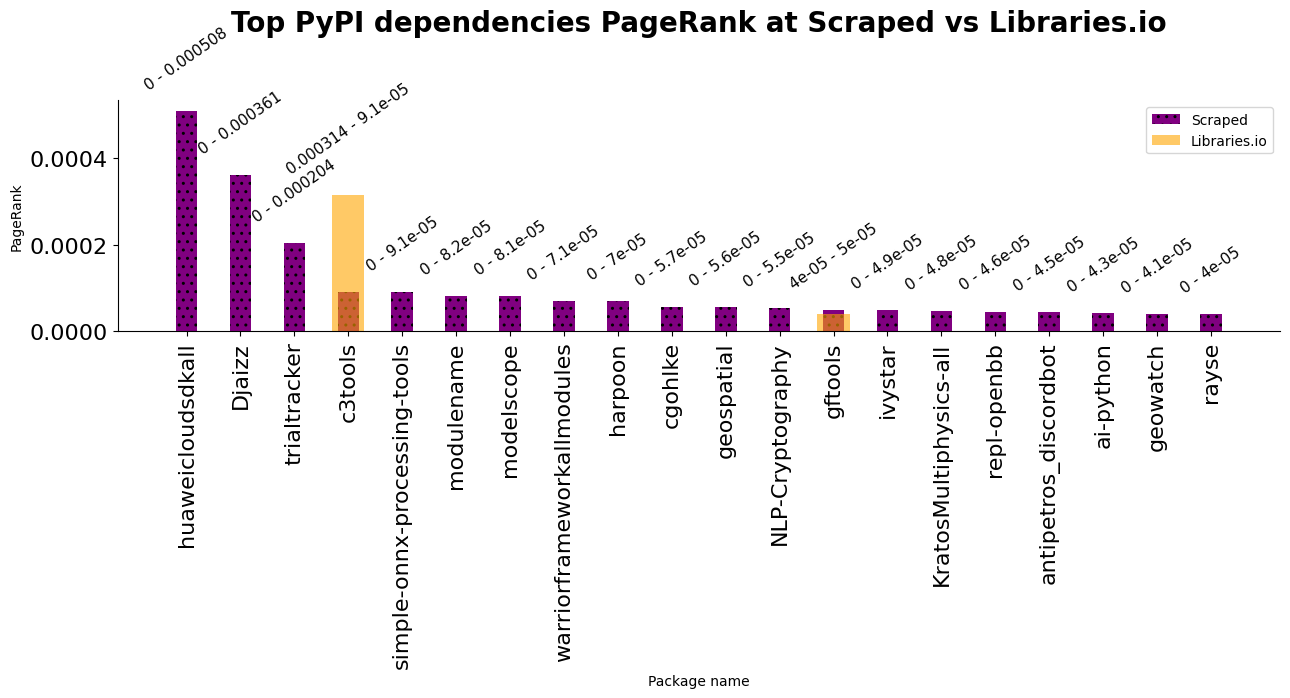
\includegraphics[width=1\textwidth]{img/pypi/t20_dep_pr_scraped.png}
        \caption{Top \textit{PageRank} en scraped}
        \label{fig:Top PageRank en scraped}
    \end{center}
\end{figure}

Al examinar el nuevo conjunto de datos, se puede observar una tendencia similar a la anterior.
El aumento en el número de paquetes se refleja en una alta frecuencia de paquetes con un bajo
PageRank. Además, se observa una disminución general del valor del \textit{PageRank} en la mayoría de
la red. Esta disminución del \textit{PageRank} puede interpretarse como una mejora en términos de
vulnerabilidad.

Una conclusión que se puede extraer es que el crecimiento en el número de paquetes ha llevado
a una mayor presencia de paquetes con un bajo PageRank. Esto sugiere que hay una mayor
proporción de paquetes menos importantes en la red.

En este top se pueden observar las conclusiones previamente mencionadas en relación a la red de
dependencias. La mayoría de los paquetes en este conjunto son nuevos, lo que ha llevado a una
disminución del \textit{PageRank} en comparación con el caso anterior. Sin embargo, es
interesante destacar que algunos paquetes, como \textit{c3tools} y
\textit{gftools},
se mantienen en el top, lo que sugiere que han resistido bien el paso del tiempo y podrían
considerarse estables en la red, a pesar de tener una mayor probabilidad de
vulnerabilidad.

Además, se puede observar que los tres paquetes principales en este conjunto tienen
un \textit{PageRank} considerablemente más alto que el resto. Esta diferencia en
el \textit{PageRank} podría indicar que estos paquetes son especialmente relevantes
en la red de dependencias\footnote{Los tres paquetes principales en este conjunto son
    altamente influyentes y desempeñan un papel crucial en la interconexión de otros paquetes
    en la red de dependencias.}.

\begin{figure}[h!]
    \begin{center}
        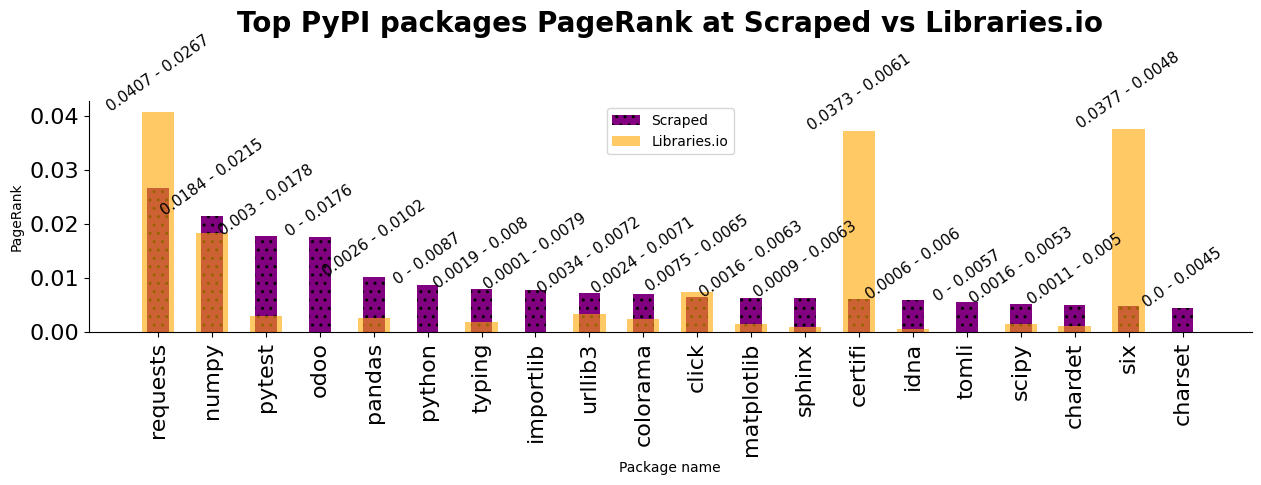
\includegraphics[width=1\textwidth]{img/pypi/t20_pkg_pr_scr.png}
        \caption{Top \textit{PageRank} paquetes en scraped}
        \label{fig:Top PageRank paquetes en scraped}
    \end{center}
\end{figure}

Si invertimos el grafo de nuestra red de dependencias \ref{fig:Top PageRank paquetes en scraped}, podemos estudiar el \textit{PageRank}
desde el punto de vista de la relevancia del paquete en la red. Un alto \textit{PageRank}
implica que el paquete tiene una cantidad significativa de enlaces entrantes desde otros paquetes
importantes. Esto sugiere que el paquete es visto como una fuente confiable de información o
recursos dentro de la red. En otras palabras, es más probable que los otros paquetes dependan
del paquete con un alto \textit{PageRank} para obtener información o llevar a cabo determinadas
tareas.

Un paquete con un alto \textit{PageRank} puede ser considerado crucial en términos de la funcionalidad
o el rendimiento de la red. Es probable que los otros paquetes dependan directa o indirectamente de
él para llevar a cabo sus propias funciones o tareas.

Como se puede ver en el top que mostramos a continuación, aparecen los paquetes más conocidos y
comúnmente usados de Python para los dos conjuntos de datos.

\subsubsection{Impacto (Impact)}

El impacto de un paquete se refiere al número de dependencias que se verían afectadas si
ocurriera un defecto en ese paquete. Esta métrica podría utilizarse para evaluar la criticidad
o importancia de un paquete en la red de dependencias y ayudar en la identificación de los
paquetes que tienen un mayor impacto en el sistema en caso de fallos.

\begin{table}[htbp]
    \centering
    \caption{Comparación entre paquetes obtenidos de libraries.io y scraped para la metrica impact}
    \begin{tabular}{ccc}
        \hline
        \textbf{libraries.io} & \textbf{scraped}   \\
        \hline
        six, 36757            & numpy, 448177      \\
        certifi, 18739        & six, 424014        \\
        requests, 17740       & python, 422180     \\
        pyparsing, 14111      & importlib, 420861  \\
        packaging, 13433      & typing, 417287     \\
        appdirs, 12619        & colorama, 416663   \\
        setuptools, 11803     & matplotlib, 414520 \\
        python-dateutil, 9825 & chardet, 413067    \\
        numpy, 7396           & Cython, 412181     \\
        pytz, 6878            & click, 411954      \\
        \hline
    \end{tabular}
\end{table}


Resulta interesante apreciar que los paquetes del top siguen siendo prácticamente los mismos
pese al notable incremento del impacto y que además esta métrica se relaciona bastante con el
Pagerank a nivel de paquete.

\begin{figure}[h!]
    \begin{center}
        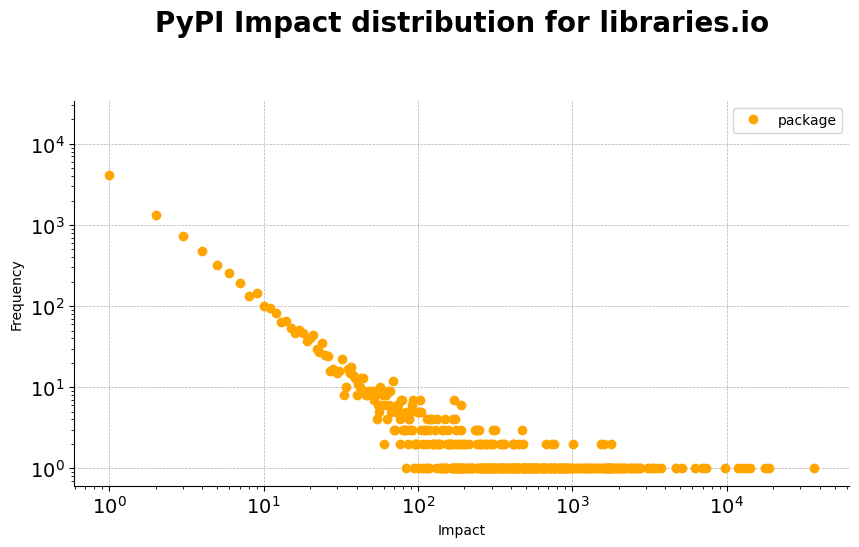
\includegraphics[width=1\textwidth]{img/pypi/librariesio_impact_distribution.png}
        \caption{Distribución del impacto en la red de libraries.io}
        \label{fig:Distribución del impacto en la red de libraries.io}
    \end{center}
\end{figure}

A la vista de la distribución del impacto en la red de libraries.io \ref{fig:Distribución del impacto en la red de libraries.io}, se observa un patrón que se
asemeja al comportamiento de la distribución del grado de salida (\textit{out degree}). Se puede notar
que existen numerosos paquetes con un impacto bajo, y la única explicación plausible es que estos paquetes
no son ampliamente utilizados como dependencias en otros paquetes.

Es común que la mayoría de los paquetes tengan un impacto relativamente bajo, en el rango de alrededor
de 10 paquetes. A medida que aumentamos el valor del impacto, la frecuencia de paquetes con un impacto
alto disminuye significativamente.

Este patrón sugiere que la mayoría de los paquetes en la red de libraries.io no tienen una influencia
crítica en las dependencias y, por lo tanto, su fallo o defecto tendría un impacto limitado en el
sistema en general. Sin embargo, se
identifican ciertos paquetes cuyo impacto es notablemente mayor, lo cual indica que son cruciales
y tienen una influencia significativa en las dependencias.

\begin{figure}[h!]
    \begin{center}
        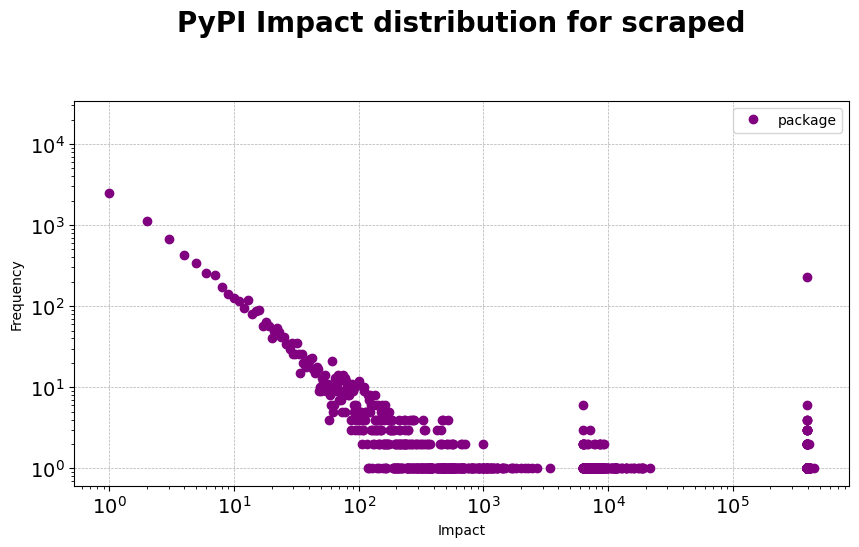
\includegraphics[width=1\textwidth]{img/pypi/scraped_impact_distribution.png}
        \caption{Distribución del impacto en la red scraped}
        \label{fig:Distribución del impacto en la red scraped}
    \end{center}
\end{figure}

Al evaluar el estado actual de la red, se observan cambios significativos en la distribución del
impacto, que muestra similitudes con la distribución del grado de salida (\textit{out degree}),
aunque también presenta variaciones y la formación de grupos con tendencias similares.

En particular, se ha observado un considerable aumento en el impacto general de los paquetes en la
red. Ahora se identifica la presencia de un número considerable de paquetes con un impacto del orden
de 10², lo cual indica que su influencia en las dependencias ha aumentado
significativamente.

Además, se distingue un segundo grupo más reducido de paquetes con un impacto alto, en el orden de 10000.
Este grupo de paquetes merece especial atención debido a su impacto significativo
en la red de dependencias.

Asimismo, se ha identificado otro grupo no existente anteriormente que resulta notable debido a
su impacto elevado.


Al analizar el incremento del impacto en la red de dependencias, se observa una distinción entre
dos casos. Por un lado, hay paquetes que han experimentado una disminución en su nivel de impacto
o han mantenido un grado de \emph{vulnerabilidad} estable a lo largo del tiempo. Por otro lado,
existen paquetes que han experimentado un aumento significativo en su impacto.

Es notable que estos paquetes que han experimentado un aumento considerable en su impacto
están interrelacionados y forman parte de componentes altamente conectados dentro de la red.
Esta \emph{interconexión} entre los paquetes permite un aumento grupal del impacto, amplificando
así la magnitud de las consecuencias en caso de fallos o defectos.

\begin{table}[htbp]
    \centering
    \caption{Comparación del incremento del impacto para de libraries.io, scraped}
    \begin{tabular}{cccc}
        \hline
        \textbf{Paquete} & \textbf{libraries.io} & \textbf{scraped} & \textbf{incremento} \\
        \hline
        numpy            & 7396                  & 448177           & 440781              \\
        importlib        & 24                    & 420861           & 420837              \\
        colorama         & 1795                  & 416663           & 414868              \\
        typing           & 2434                  & 417287           & 414853              \\
        matplotlib       & 748                   & 414520           & 413772              \\
        Cython           & 75                    & 412181           & 412106              \\
        chardet          & 1707                  & 413067           & 411360              \\
        BeautifulSoup4   & 75                    & 411391           & 411316              \\
        genshi           & 5                     & 411290           & 411285              \\
        cssselect        & 260                   & 411490           & 411230              \\
        \hline
    \end{tabular}
\end{table}


A la vista del top de incremento del impacto se aprecia similitud entre los paquetes seleccionados,
los cuales resultan muy familiares para los desarrolladores que usamos el lenguaje Python ya que
son paquetes muy usados en casi todo tipo de software.

Si analizamos el decremento se puede ver que no es tan acentuado como el incremento, no
podemos sacar muchas conclusiones de ello más que estos paquetes han disminuido el número de
dependencias transitivas que poseían, simplemente quedémonos con observar la tendencia y ver qué
paquetes han sido los más afectados.

\begin{table}[htbp]
    \centering
    \caption{Disminución del impacto en libraries.io y scraped}
    \begin{tabular}{cccc}
        \hline
        \textbf{Paquete}              & \textbf{librariesio} & \textbf{scraped} & \textbf{incremento} \\
        \hline
        python-dateutil               & 9825                 & 0                & -9825               \\
        importlib-metadata            & 4677                 & 0                & -4677               \\
        backports.functools-lru-cache & 1944                 & 0                & -1944               \\
        async-timeout                 & 1828                 & 0                & -1828               \\
        asn1crypto                    & 2503                 & 817              & -1686               \\
        oslo.i18n                     & 1503                 & 0                & -1503               \\
        futures                       & 2277                 & 816              & -1461               \\
        oslo.utils                    & 1242                 & 0                & -1242               \\
        singledispatch                & 1213                 & 87               & -1126               \\
        pyasn1-modules                & 1101                 & 0                & -1101               \\
        \hline
    \end{tabular}
\end{table}




\subsubsection{Reach}

La métrica llamada \emph{Reach} , que se refiere a la vulnerabilidad
frente a fallos en una red de paquetes, se utiliza para medir el alcance de los paquetes afectados
por un fallo aleatorio en la red. Se define como la media aritmética del alcance de los nodos
en la red.

La vulnerabilidad de la red se cuantifica al calcular el número esperado de paquetes comprometidos
por un fallo aleatorio, asumiendo que las probabilidades de fallo son independientes y siguen
una distribución uniforme.

A nivel de paquete se refiere al número de paquetes que se verían afectados por un fallo en un
paquete o alguna de sus dependencias transitivas\footnote{El alcance a nivel de paquete se
    define como el número de paquetes que se verían afectados por un fallo en un paquete o alguna
    de sus dependencias transitivas.}.

\begin{figure}[h!]
    \begin{center}
        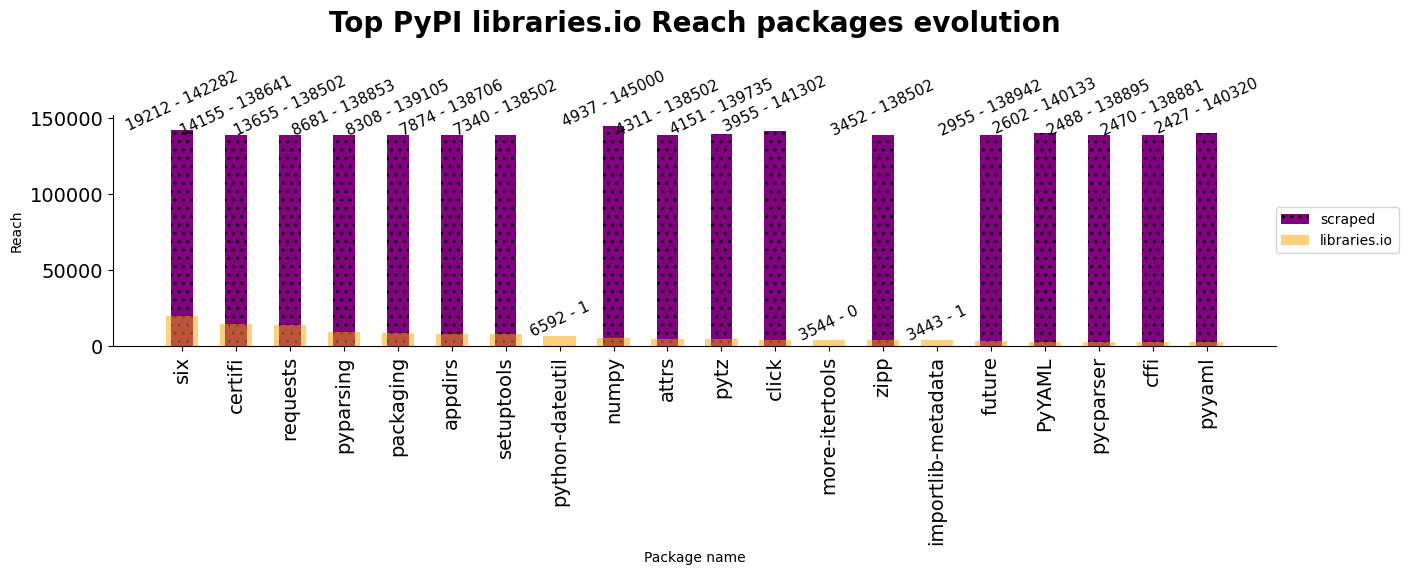
\includegraphics[width=1\textwidth]{img/pypi/top_librariesio_reach_evolution.png}
        \caption{Top Reach en libraries.io}
    \end{center}
\end{figure}


Bajo esta definición, al analizar el top 20 de paquetes con el mayor \textit{Reach} en una red compuesta por aproximadamente 40000 nodos, resulta llamativo observar que algunos paquetes
presentan un \textit{Reach} tan elevado. Además, es importante destacar que estos paquetes se
encuentran entre los más populares y utilizados en Python, lo cual justifica el valor alcanzado.
Sin embargo, desde el punto de vista de la vulnerabilidad de la red, resulta preocupante, ya que
un fallo en alguno de estos paquetes representaría un peligro significativo.

En relación a estos paquetes, en el estado actual de la red, resulta sorprendente el incremento
que han experimentado en su alcance. Este incremento puede ser explicado por el crecimiento en el
número de nodos de la red. Estos valores destacados para los paquetes en cuestión nos proporcionan
una idea clara de la vulnerabilidad que introduce su presencia en la red. Si consideramos que
\textit{PyPI} actualmente cuenta con aproximadamente \textit{200000} paquetes, un fallo en alguno de estos paquetes
que se encuentran en el \textit{top} del ranking tendría un impacto \textit{considerable} en la integridad de la red.


\begin{figure}[h!]
    \begin{center}
        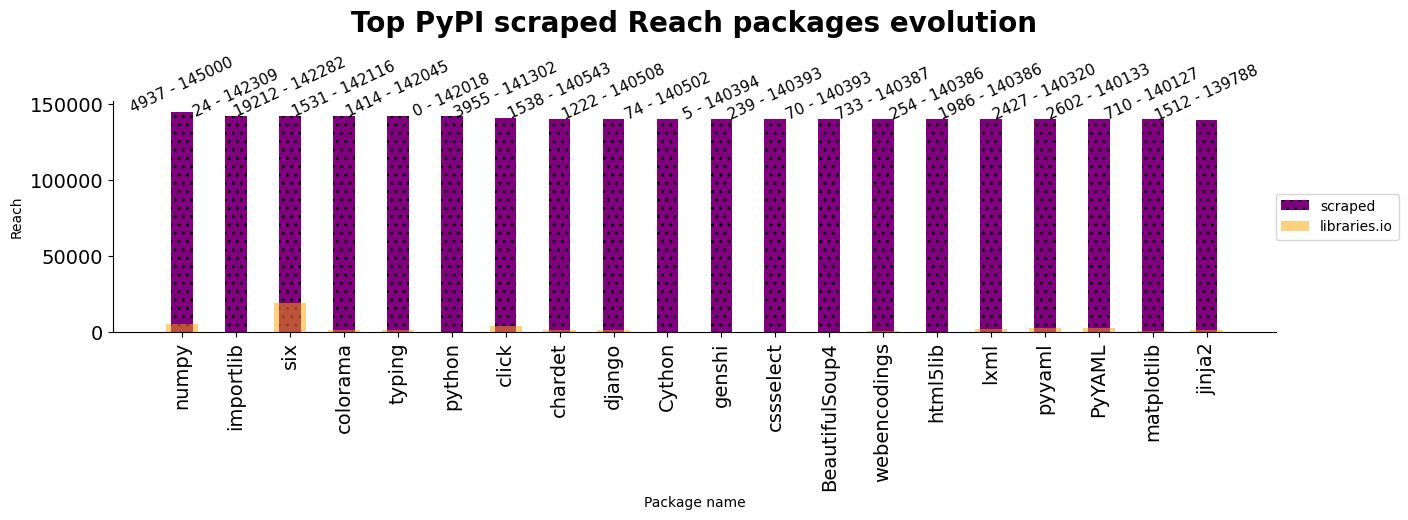
\includegraphics[width=1.2\textwidth]{img/pypi/top_scraped_reach_evolution.png}
        \caption{Top Reach en scraped}
    \end{center}
\end{figure}


Si comparamos las distribuciones de \textit{reach} para los dos conjuntos de datos, podemos ver que tienen una
tendencia similar a la distribución de \textit{grado de salida}.

\begin{figure}[h!]
    \begin{center}
        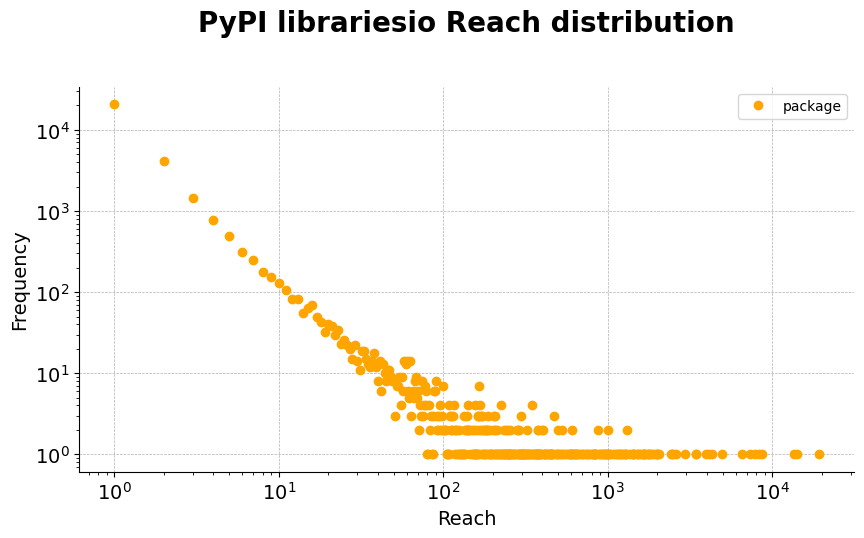
\includegraphics[width=0.8\textwidth]{img/pypi/librariesio_reach_distribution.png}
        \caption{Distribución del Reach en libraries.io}
    \end{center}
\end{figure}

\begin{figure}[h!]
    \begin{center}
        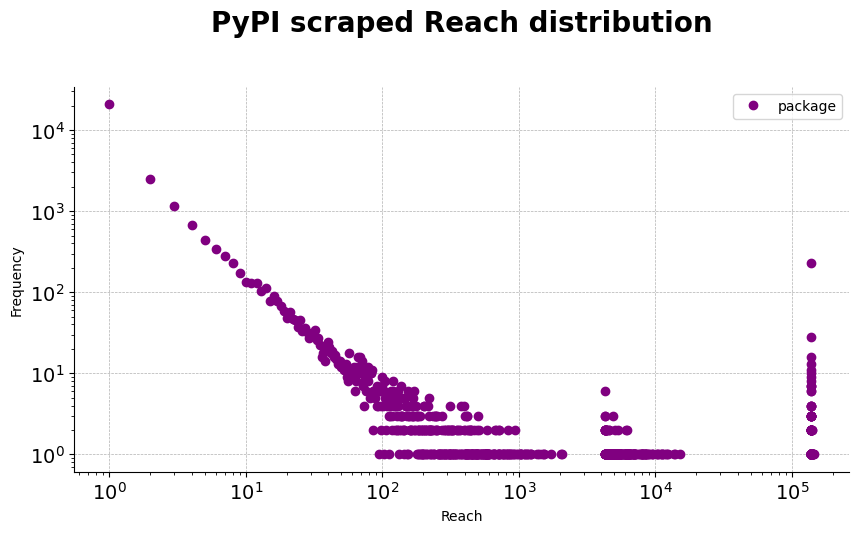
\includegraphics[width=0.8\textwidth]{img/pypi/scraped_reach_distribution.png}
        \caption{Distribución del Reach en scraped}
    \end{center}
\end{figure}

El nuevo conjunto de datos muestra la existencia de tres grupos distintos. El primer grupo presenta
un valor de \textit{Reach} bajo, lo que indica que no hay un nivel significativo de vulnerabilidad. En el
segundo grupo, el valor de \textit{Reach} se sitúa en el orden de \textit{10000}, lo cual representa un riesgo mayor.
Aunque el número de paquetes pertenecientes a este grupo no es excesivamente alto, es importante
tenerlo en cuenta debido a su nivel de vulnerabilidad. Por último, el tercer grupo se caracteriza
por tener un valor de \textit{Reach} muy alto.

Según mi interpretación, estos dos grupos de alto Reach representan nodos pertenecientes a componentes
fuertemente conexos y son en los que habría que poner el foco para proteger la estabilidad de la red.

\begin{figure}[h!]
    \begin{center}
        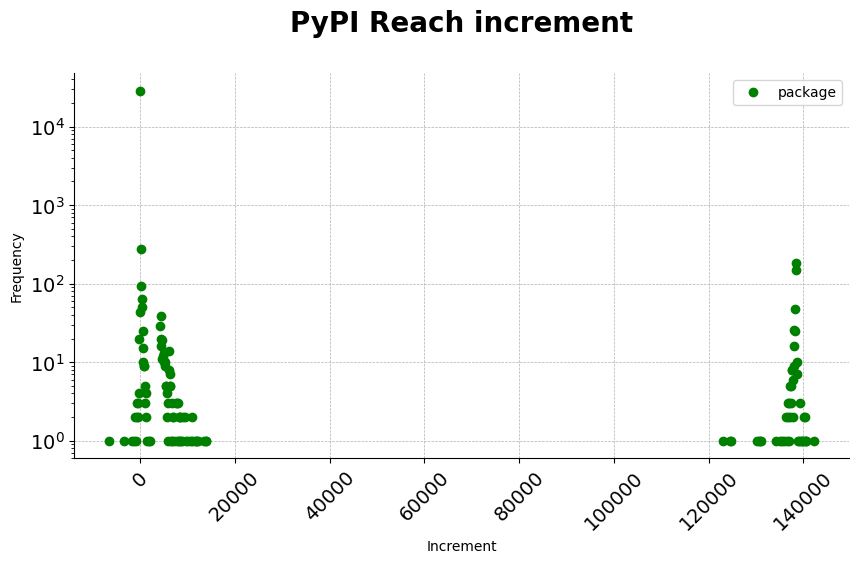
\includegraphics[width=0.8\textwidth]{img/pypi/reach_increment.png}
        \caption{Incremento del Reach}
    \end{center}
\end{figure}

En relación al incremento del Reach, se pueden identificar dos tendencias distintas. En la primera
tendencia, se observa que el Reach se mantiene relativamente estable, con fluctuaciones dentro de un
rango aproximado de ±15,000. Por otro lado, el segundo grupo exhibe un notable aumento en el valor
del Reach. Un fallo en un paquete perteneciente a este grupo podría generar graves problemas en la red.
Este incremento puede ser atribuido al crecimiento en el número de nodos de la red. Como resultado de
este crecimiento, han surgido dependencias transitivas que han contribuido significativamente a este
aumento considerable en el Reach.

\subsubsection{Componente fuertemente conexo}

En un \textit{componente fuertemente conexo}, todos los nodos están directa o indirectamente conectados
entre sí. No importa si los caminos son directos o implican múltiples pasos a través de otros nodos,
lo fundamental es que existe una ruta dirigida desde cualquier nodo al resto de los nodos del componente.

Bajo la red de libraries.io no se identifican componentes fuertemente conexos. Esto se debe principalmente
al tamaño de la red, que es relativamente pequeño. Sin embargo, en el nuevo conjunto de datos, se ve claramente
la existencia de componentes fuertemente conexos.

    \begin{tabular}{|c|c|c|c|c|c|c|c|}
        \hline
        Size & Avg    & Density & Diameter & Clustering & Transitive \\
             & degree &         &          & coefficient      & dependencies       \\
        \hline
        283  & 8.890  & 0.015   & 14       & 0.196      & 206873     \\
        9    & 4.947  & 0.137   & 8        & 0.358      & 23807      \\
        8    & 3.000  & 0.214   & 6        & 0.222      & 6288       \\
        8    & 5.250  & 0.375   & 3        & 0.383      & 6784       \\
        8    & 4.750  & 0.339   & 5        & 0.498      & 6752       \\
        6    & 5.000  & 0.500   & 2        & 0.776      & 4536       \\
        6    & 4.666  & 0.466   & 3        & 0.470      & 4452       \\
        6    & 3.666  & 0.366   & 3        & 0.448      & 4440       \\
        5    & 2.800  & 0.350   & 4        & 0.000      & 3770       \\
        5    & 6.000  & 0.750   & 2        & 0.777      & 3855       \\
        5    & 3.200  & 0.400   & 4        & 0.386      & 3765       \\
        5    & 3.600  & 0.450   & 3        & 0.421      & 3755       \\
        4    & 3.000  & 0.500   & 3        & 0.406      & 5276       \\
        4    & 2.500  & 0.416   & 3        & 0.000      & 3016       \\
        4    & 3.000  & 0.500   & 3        & 0.406      & 3220       \\
        4    & 3.000  & 0.500   & 3        & 0.700      & 2988       \\
        4    & 3.000  & 0.500   & 3        & 0.406      & 3048       \\
        4    & 3.000  & 0.500   & 3        & 0.406      & 3064       \\
        4    & 4.500  & 0.750   & 2        & 0.800      & 2948       \\
        3    & 2.666  & 0.666   & 2        & 0.000      & 3780       \\
        \hline
    \end{tabular}

A partir de estos datos, se pueden extraer varias conclusiones. Existen componentes fuertemente conexos de diversos
tamaños, desde pequeños hasta muy grandes. Algunos componentes tienen una alta importancia medida por el pagerank
del nodo principal. La densidad y el coeficiente de agrupamiento varían entre los componentes, lo que sugiere diferentes
patrones de conexiones. Además, el número de dependencias transitivas varía ampliamente en funcion del tamaño del componente.

\begin{figure}[h!]
    \begin{center}
        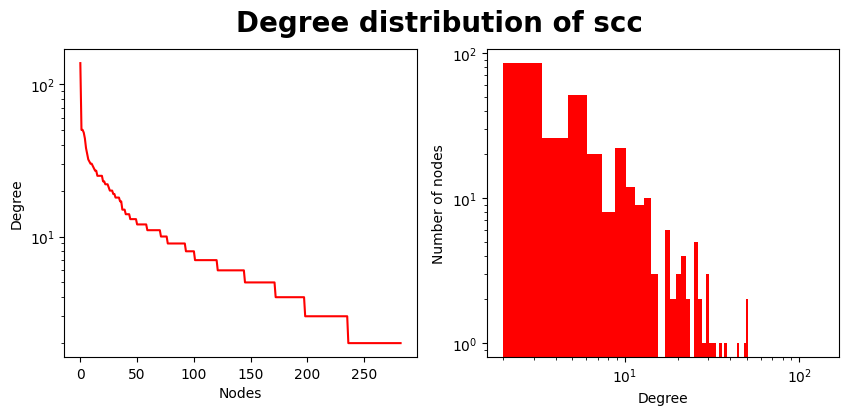
\includegraphics[width=1\textwidth]{img/pypi/scc1_dist.png}
        \caption{Distribucion de grado del mayor componente fuertemente conexo}
    \end{center}
\end{figure}

\begin{figure}[h!]
    \begin{center}
        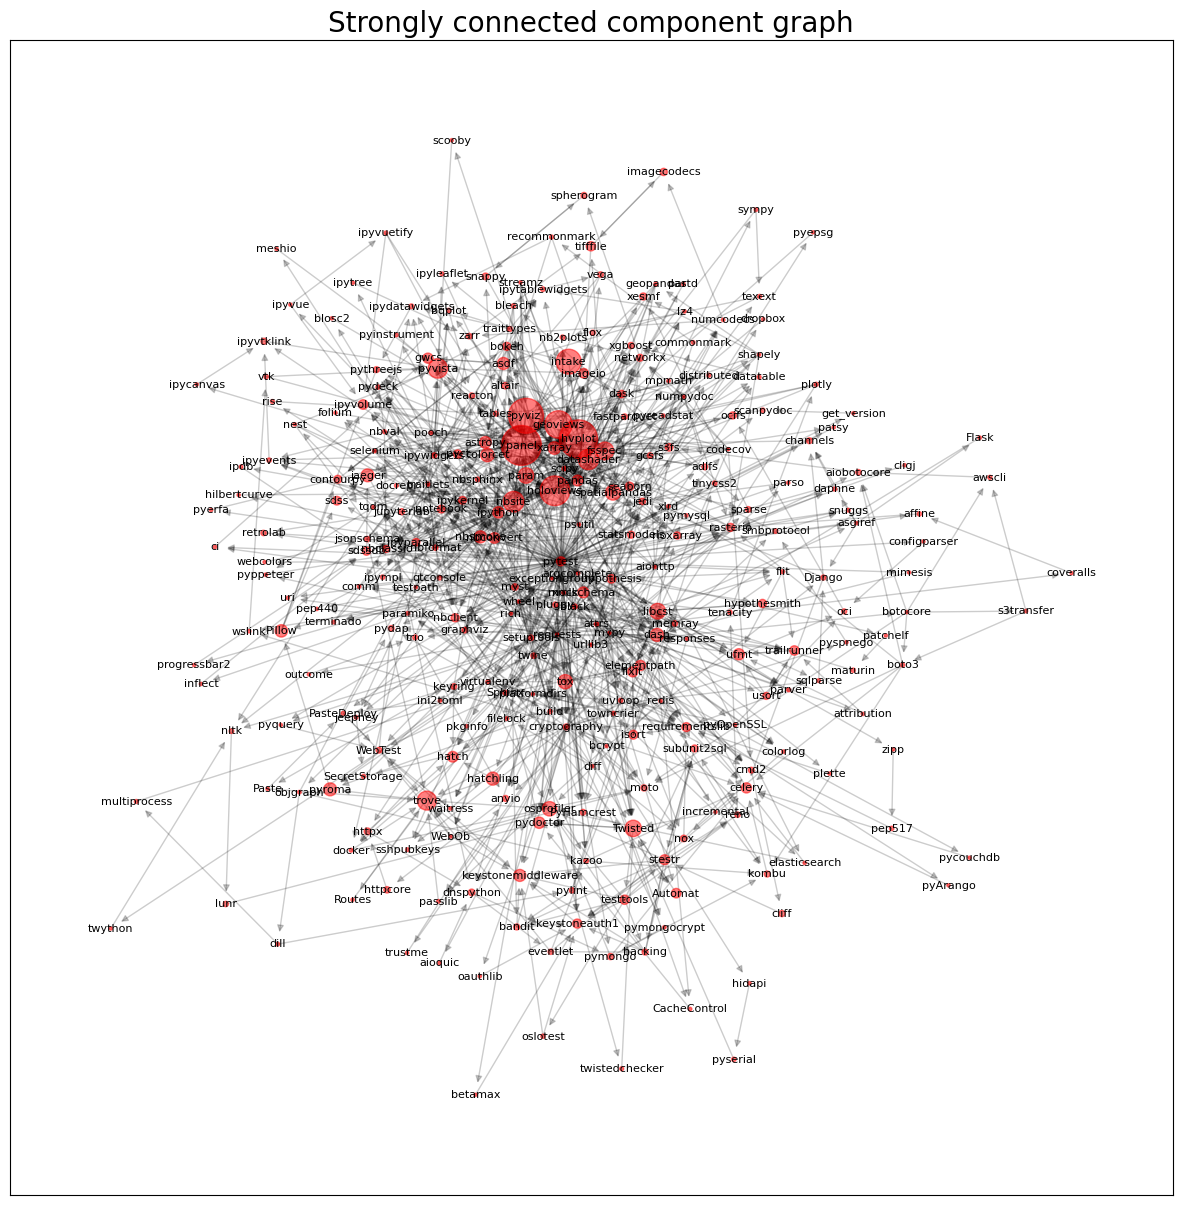
\includegraphics[width=1.2\textwidth]{img/pypi/scc1.png}
        \caption{Mayor componente fuertemente conexo}
    \end{center}
\end{figure}

